26. $(|x|-3)(x+|y|-1)=0\Leftrightarrow \left[\begin{array}{l} |x|-3=0,\\ x+|y|-1=0.\end{array}\right.\Leftrightarrow\left[\begin{array}{l} x=3,\\ x=-3,\\ y=1-x,\ x\leqslant1,\\ y=x-1,\ x \leqslant1.\end{array}\right.$
$$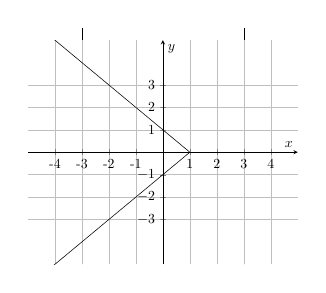
\begin{tikzpicture}[scale=0.5]
\tikzset {line01/.style={line width =0.3pt}}
\draw[line01] (1.38,0) -- (1.38,6);
\draw[line01] (5.5,0) -- (5.5,6);
\begin{axis}[
    axis lines = middle,
    grid=major,
    legend pos={south west},
    xlabel = {$x$},
    %xlabel style={below right},
    ylabel = {$y$},
    xmin=-5,
    xmax=5,
    ymin=-5,
    ymax=5,
    xtick={-4, -3, -2,-1,1, 2,3,4},
    xticklabels={-4,-3, -2,-1,1, 2,3, 4},
    ytick={1,-1,-3,3,-2,2},
     %yticklabels={-5,-4,$ $,$-\frac{3}{2}$,6},
                  ]
	\addplot[domain=-5:1, samples=100, color=black] {1-x};
    \addplot[domain=-5:1, samples=100, color=black] {x-1};

	%\addlegendentry{$\text{Рис. 1}$};
\end{axis}
%\draw (3.7,3.05) circle (2pt);
\end{tikzpicture}$$
